% Section content template for individual Educative lessons
% This file contains the actual content for a specific section
% Generated from Educative API section content

% Section: Trade-Offs in Databases
% Section ID: 5531655174881280
% Section Slug: trade-offs-in-databases
% Generated: 2025-12-06T21:15:15.745766

\subsection{Which is the best database sharding approach?}\label{yZXpLx2rhbuKn_JN-nLhL}
\\
Both horizontal and vertical sharding involve adding resources to our computing infrastructure. Our business stakeholders must decide which is suitable for our organization. We must scale our resources accordingly for our organization and business to grow, to prevent downtime, and to reduce latency. We can scale these resources through a combination of adjustments to CPU, physical memory requirements, hard disk adjustments, and network bandwidth.\\
\strut \\
The following sections explain the pros and cons of centralized and distributed databases:

\subsection{Advantages and disadvantages of a centralized database}\label{UwsBl0ukWeQln5m_zv3K9}

\subsubsection{Advantages}\label{v_bHQ0K0zIqqrfCt0V3di}

\begin{itemize}
\item
\protect\phantomsection\label{JKx-vff9zBdUnwxP4lTTO}
Data maintenance, such as updating and taking backups of a centralized database, is easy.
\item
\protect\phantomsection\label{Wy890jXtO79KmI-VYakL2}
Centralized databases provide stronger consistency and ACID transactions than distributed databases.
\item
\protect\phantomsection\label{twVL2h0YYWg6_rLcJno_Z}
Centralized databases provide a much simpler programming model for the end programmers as compared to distributed databases.
\item
\protect\phantomsection\label{2XwFp2k7s2b_jEamdqzt5}
It's more efficient for businesses that have a small amount of data to store that can reside on a single node.
\end{itemize}

\subsubsection{Disadvantages}\label{QIz1EDJUUaduBB3OwvCQO}

\begin{itemize}
\item
\protect\phantomsection\label{daJs-Gi98PioErF3SC6D6}
A centralized database can slow down, causing high latency for end users, when the number of queries per second accessing the centralized database is approaching single-node limits.
\item
\protect\phantomsection\label{r26_IJGxr7pT-inGrY3u1}
A centralized database has a single point of failure. Because of this, its probability of not being accessible is much higher.
\end{itemize}

\subsection{Advantages and disadvantages of a distributed database}\label{cLS69ijfM-ME26FoRzpVI}

\subsubsection{Advantages}\label{UPaZ9UQWrDd90WmlHV3jD}

\begin{itemize}
\item
\protect\phantomsection\label{wqaBuD18kQuWx4pvShYTB}
It's fast and easy to access data in a distributed database because data is retrieved from the nearest database shard or the one frequently used.
\item
\protect\phantomsection\label{70f98z_F6m9lWDXbBjFGa}
Data with different levels of distribution transparencyDistributionTransparency can be stored in separate places.
\item
\protect\phantomsection\label{wbGLzdC-xGA-6-i0TSEWU}
Intensive transactions consisting of queries can be divided into multiple optimized subqueries, which can be processed in a parallel fashion.
\end{itemize}

\subsubsection{Disadvantages}\label{N14Kxfstw-hd1CAU-NCT4}

\begin{itemize}
\item
\protect\phantomsection\label{8D49sv9lcIYFVFf-L6ly1}
Sometimes, data is required from multiple sites, which takes more time than expected.
\item
\protect\phantomsection\label{SQ_qvJhYk2lWi_EM0FrF1}
Relations are partitioned vertically or horizontally among different nodes. Therefore, operations such as joins need to reconstruct complete relations by carefully fetching data. These operations can become much more expensive and complex.
\item
\protect\phantomsection\label{dPhxVyPaPTGL0llbncTmM}
It's difficult to maintain consistency of data across sites in the distributed database, and it requires extra measures.
\item
\protect\phantomsection\label{9_ec9xYpGI18NaIm5yTKI}
Updations and backups in distributed databases take time to synchronize data.
\end{itemize}

\subsection{Query optimization and processing speed in a distributed database}\label{4AqVVyVRmxRG-QzI6dCB9}
\\
A transaction in the distributed database depends on the type of query, number of sites (shards) involved, communication speed, and other factors, such as underlying hardware and the type of database used. However, as an example, let's assume a query accessing three tables, \texttt{Store}, \texttt{Product}, and \texttt{Sales}, residing on different sites.
\\
The number of attributes in each table is given in the following figure:

\begin{figure}[htbp]
 \centering
 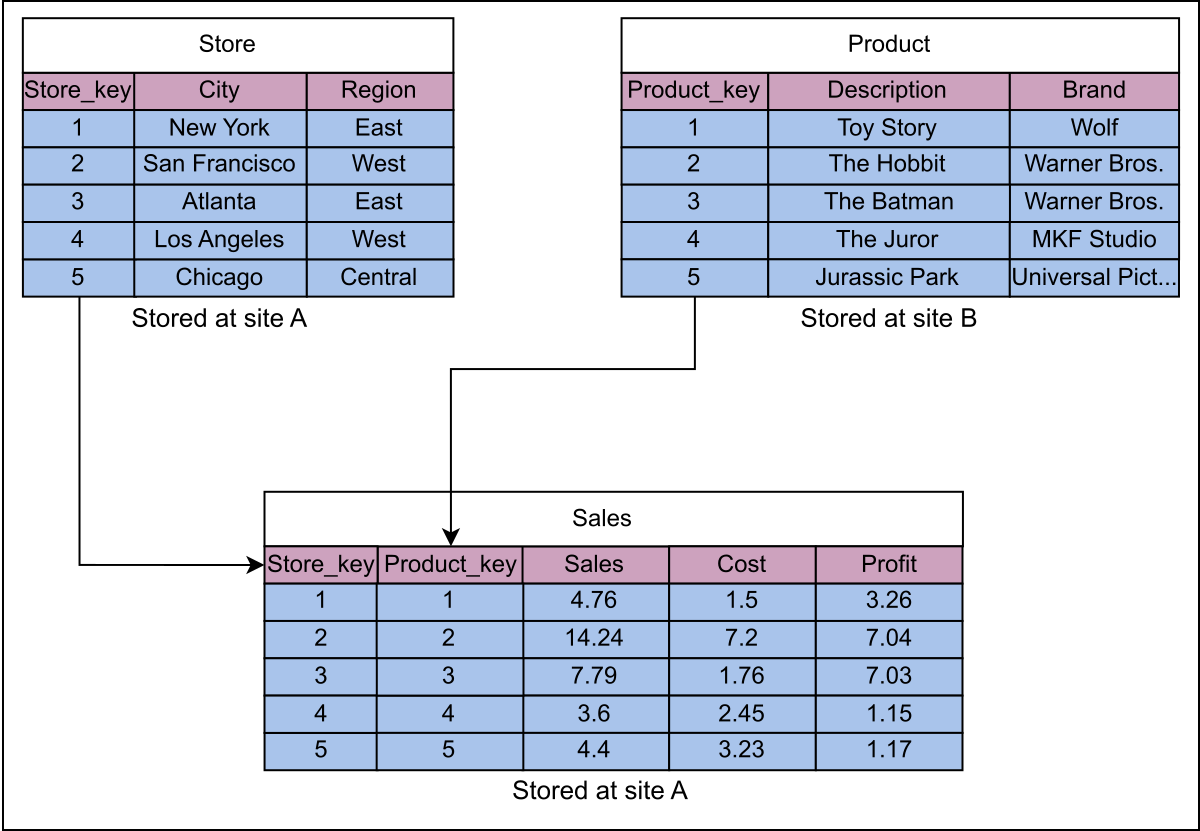
\includegraphics[width=0.5\textwidth]{Images/chapter_9/section_5531655174881280/4877851539275776.png}
 \caption{Database schema consisting of three tables: Store, Product, and Sales}
\end{figure}

Let's assume the distribution of both tables on different sites is the following:

\begin{itemize}
\item
\protect\phantomsection\label{WBUQmuTZIY_cNTEDCxxAO}
The \texttt{Store} table has 10,000 tuples stored at site A.
\item
\protect\phantomsection\label{HB8Wo7LIF9vhsWuuvRo4W}
The \texttt{Product} table has 100,000 tuples stored at site B.
\item
\protect\phantomsection\label{6Ugy-EqzYKj9cxZ9wckjA}
The \texttt{Sales} table has one million tuples stored at site A.
\end{itemize}
\\
Now, assume that we need to process the following query:

\begin{itemize}
	\item Keeps data geographically close to your users, thus reducing access latency.
	\item Allows the system to continue working even if some of its parts have failed, thus increasing availability.
	\item Scales out the number of machines that can serve read queries, thus increasing read throughput.
\end{itemize}
\\
\\
The above query performs the join operations on the \texttt{Store}, \texttt{Sales}, and \texttt{Product} tables and retrieves the Store\_key values from the table generated in the result of join operations.
\\
Next, assume every stored tuple is 200 bits long. That's equal to 25 Bytes. Furthermore , estimated cardinalities of certain intermediate results are as follows:

\begin{itemize}
\item
\protect\phantomsection\label{JV4c-NXEA7Buhf2BIa1Ia}
The number of the \texttt{Wolf} brand is 10.
\item
\protect\phantomsection\label{tovkUEjFcJHYl0iKClv0y}
The number of \texttt{East} region stores is 3000 (since there are 10,000 rows in the store table, and 3000 have region as east).
\end{itemize}
\\
Communication assumptions are the following:

\begin{itemize}
\item
\protect\phantomsection\label{tCq3ZX_8wzp8Sn7kZKVW5}
Data rate \protect\phantomsection\label{katex_inline_yc4key1mImkGZMuZ1q3IJ}{{{\(=\)}}} 50M bits per second
\item
\protect\phantomsection\label{WwUOqkXgVziWti8B0Vbuc}
Access delay \protect\phantomsection\label{katex_inline_RUPpsgwLM0tmWecf8-POj}{{{\(=\)}}} 0.1 second
\end{itemize}

\subsubsection{Parameters assumption}\label{RGUVUjZxoLW-EkbEo-u6v}
\\
Before processing the query using different approaches, let's define some parameters:
\\
\protect\phantomsection\label{katex_inline_tJIMUN8gwTd1Con09sRTy}{{{\(a =\)}}} Total access delay
\\
\protect\phantomsection\label{katex_inline_Ilmaa5HgwNDhXy56PTLUt}{{{\(b=\)}}} Data rate
\\
\protect\phantomsection\label{katex_inline_SmlphuImG1oNYGUZsMENJ}{{{\(v =\)}}} Total data volume
\\
Now, let's compute the total communication time, \protect\phantomsection\label{katex_inline_uz5SI3ugaA23Eh8AwbMZc}{{{\(T\)}}}, according to the following formula:

\[
T = a + \frac{v}{b}
\]

Let's try the following possible approaches to execute the query.

\subsubsection{Possible approaches}\label{5qVBl3nAwX0STNMPMwD4H}

\begin{itemize}
\item
\protect\phantomsection\label{G38WxQ4QlAUKGjZV5l1wt}
Move the \texttt{Product} table to site A and process the query at A.
\end{itemize}

\[
\text{T} = 0.1 + \frac{100,000 \times 200}{50,000,000} = 0.5 \ \text{seconds}
\]

Here, 0.1 is the access delay of the table on site A, and 100,000 is the number of tuples in the \texttt{Product} table. The size of each tuple in bits is 200, and 50,000,000 is the data rate. The 200 and 50,000,000 figures are the same for all of the following calculations.

\begin{itemize}
\item
\protect\phantomsection\label{1YqIFP3qr5emOkE9RPS-u}
Move \texttt{Store} and \texttt{Sales} to site B and process the query at B:
\end{itemize}

\[
\text{T} = 0.2 + \frac{(10,000 + 1,000,000) \times 200}{50,000,000} = 4.24 \ \text{seconds}
\]

Here, 0.20.1 second each for the Product and Store tables, hence 0.1 + 0.1 = 0.2 is the access delay of the \texttt{Store} and \texttt{Sales} tables. The numbers 10,000 and 1,000,000 are the number of tuples in the \texttt{Store} and \texttt{Sales} tables, respectively.

\begin{itemize}
\item
\protect\phantomsection\label{eh7pHTOeTfCiznIaURPNb}
Restrict \texttt{Brand} at site B to \texttt{Wolf} (called selectionThe select operation accepts a relation as input and produces a subset of the tuples from that relation that meet a selection predicate. The predicate operates as a type of filter, and we can utilize both conjunctions and disjunctions to merge multiple predicates.) and move the result to site A:
\end{itemize}

\[
\text{T} = 0.1 + \frac{10 \times 200}{50,000,000} \approx 0.1 \ \text{seconds}
\]

Here, 0.1 is the access delay of the \texttt{Product} table. The number of the \texttt{Wolf} brand is 10, hence the number of tuples.
\\
When we compare the three approaches, the third approach provides us the least latency (0.1 seconds). We didn't calculate filtering at site A because the number of rows will be much larger, and hence data volume will be more than the third case (filtering at the site B and then fetching data). This example shows that careful query optimization is also critical in the distributed database.

\subsubsection{Conclusion}\label{qIrI4MHCx9k9slC4A72D5}

Data distribution (vertical and horizontal sharding) across multiple nodes aims to improve the following features, considering that the queries are optimized:

\begin{itemize}
\tightlist
\item
Reliability (fault-tolerance)
\item
Performance
\item
Balanced storage capacity and dollar costs
\end{itemize}
\\
Both centralized and distributed databases have their pros and cons. We should choose them according to the needs of our application.



% End of section content